\section{Robust Models}

We model using a robust fit from the `robust' package, and the lmRob function \citep{RobustModels}. This fits a `robust model' which is less sensitive to outliers than a regular least squares, linear fit. The function lmRob automatically chooses an appropriate algorithm to efficiently fit a model.  The default fitting method is the so called `data-dependent algorithm'.

 \vspace{12pt}

 Again, we used median TCT as our response variable. Initially, we fit a simple robust model, lr, to our response variable, Median TCT, with  a single input predictor, Log2(Biomass). Next, we fit two multiple linear models. lrparallel.tfac is a multiple linear model with the two predictors Log2(Biomass) and tank. Finally, we fit  lrfull.tfac, that incorporates both Log2(Biomass) and tank as well as the interaction between Log2(Biomass) and tank. 

 \vspace{12pt}

%\begin{table}[H]
%\begin{singlespace*}
%\verbatiminput{tablesandimages/lr.txt}
%\caption{Model: lr}
%\label{fig:robust1}
%\end{singlespace*}
%\end{table}


\begin{table}[H]
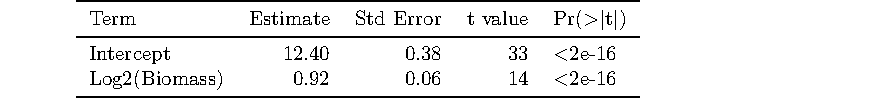
\includegraphics{Chapter3Images/robust1.pdf}
\caption{Parameter estimates and standard error for our simple robust model: lr. The $R^{2}$ value is 0.546.}
\label{fig:robust1}
\end{table}

 Table~\ref{fig:robust1} provides the results of fitting a simple linear model for median TCT using lmRob. For a unit increase in log2(biomass) this model predicts an increase in 0.925 for median TCT. This also makes sense, as Log2(Biomass) increases, we expect that the volume of eDNA in the tank will increase, and hence CT will decrease (and TCT will increase).The p-value for both intercept and Log2(Biomass) are extremely low, indicating that both  play an important role in the model. The estimates for the intercept in both the robust and linear model are quite similar.  The estimate for Log2(Biomass) is slightly less for the robust fit. We then fit a robust model for median TCT that includes biomass as a predictor and also considers tank as a possible predictor.

 \vspace{12pt}




\begin{table}[H]
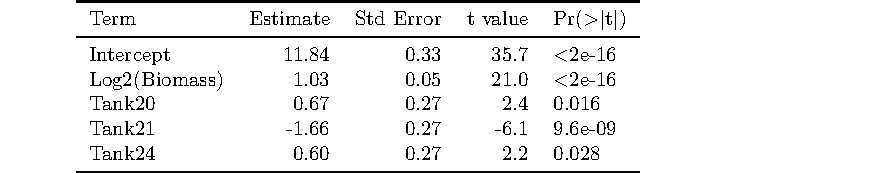
\includegraphics{Chapter3Images/robust2.pdf}
\caption{Parameter estimates and standard errors for the model lrparallel.tfac. The $R^{2}$ value is 0.619.}
\label{fig:robust2}
\end{table}



Table~\ref{fig:robust2} summarizes the model lrparallel.tfac.  For this model, lmRob produces similar conclusions for both the intercept and for the Log2(Biomass).   However, we now also have estimates for the tank. The data indicates that compared to the baseline of tank 19, tank 20 and 24 produce slightly higher median TCT estimates, while on the other hand Tank 21 produced lower TCT. These differences are possibly due to differences in bleaching and cleaning of the tanks.

 \vspace{12pt}

Finally, we fit a robust model (lrfull.tfac) for the response median TCT that includes biomass, tank, and the possible interactions between biomass and tank.

\vspace{12pt}



\begin{table}[H]
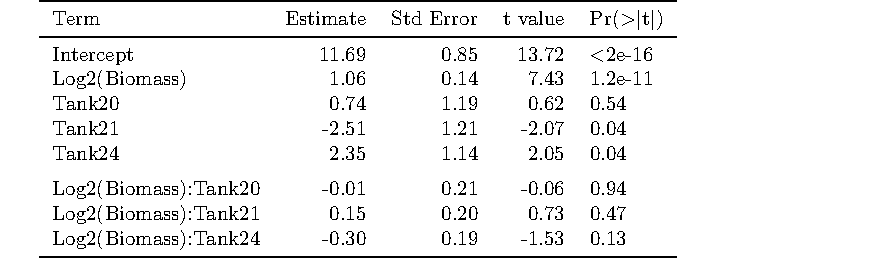
\includegraphics{Chapter3Images/robust3.pdf}
\caption{Parameter estimates and standard errors for the model lrfull.tfac. The $R^{2}$ value is 0.649.}
\label{fig:robust3}
\end{table}

 \vspace{12pt}

Table~\ref{fig:robust3} summarizes the estimates of lrfull.tfac. The robust model, lrfull.tfac containing Log2(Biomass), tank and their interaction terms produces similar results to lrparallel.tfac.
 The multiple $R^{2}$ for this model is only slightly larger than lrparallel.tfac at 0.649. The interaction terms between tank and Log2(Biomass) are not significant.  We confirmed this with an `anova' test (additional sum of squares) using the built in R function. 
  
\vspace{12pt}


 Recall that anova compares a variety of nested models. Our first model is lr, which included Log2(Biomass). Our second model, lrparallel.tfac includes for Log2(Biomass) and tank. 
 



\begin{table}[H]

\includegraphics{Chapter3Images/robustanova.pdf}
\caption{Table of results for comparing the robust models using a Robust ANOVA.}
\label{fig:robustanova}
\end{table}

Table~\ref{fig:robustanova} is the results of applying an anova test to our robust models. We do not reject the hypothesis (at the 0.05 significance level) that the interaction term is zero. We do reject the null hypothesis that the tank term is zero.















